The Seismic Sources System is the ensemble of one or several 
Initial Seismic Sources models and the Seismic Sources Logic
Tree.

The Initial Seismic Sources Model is a list of seismic sources 
(the typologies of sources admitted is described in Section
\ref{hazard:seismic_source_types}); each source is characterized
by default parameters.
%
Usually, a seismic sources model contains one or several seismic 
sources accounting for distributed seismicity (e.g. area sources, 
grid sources) and - eventually - one or several individual seismic 
sources.

The Seismic Sources Logic Tree describes the epistemic uncertainties 
associated with the parameters used to characterize the Initial 
Seismic Sources models. 
% 
Though this logic tree the user can take into account the epistemic
uncertainties associated with almost all the parameters characterizing
each source typology. 
% 
Currently OpenQuake contains just a limited number of logic tree
branch set types. 

%  - - - - - - - - - - - - - - - - - - - - - - - - - - - - - - - - - - - - - - -
\subsubsection{Seismic Sources Logic Tree}
\label{hazard:source_model_logic_tree}
\index{Logic Tree!Seismic Sources}
%
In the current version of OpenQuake, a seismic sources logic tree can be 
defined according to the following schema:
\begin{itemize}
\item The first branching level is assumed describing one or more "alternative" 
initial seismic source models.
\item Subsequent branching levels define source parameters uncertainties. 
Parameters uncertainties are applied independently to each seismic source 
in a source model. That is epistemic uncertainties are assumed uncorrelated 
between different seismic sources.
\item One branch set can be defined for branching level, thus assuming 
symmetric logic tree definition only.
\end{itemize}
%
The possibility of defining multiple source models in the first branching 
level responds to the need of modern PSHA of considering alternative source 
models (as derived by different expert opinions, for instance). 
%
Subsequent branching levels define the epistemic uncertainties that 
apply to parameters characterizing seismic sources. The  
epistemic uncertainties related to these parameters are implemented as 
\emph{rules}, that is as algorithms describing how this parameter has to be 
modified. 
%
The major advantage of using a rule-based approach is that a user does not 
need to a provide an input file containing a source model definition 
corresponding to a specific epistemic uncertainty, that is instead computed 
and applied on the fly to the initial model.
%
% ..............................................................................
% . . . . . . . . . . . . . . . . . . . . . . . . . . . . . . . . . . . > Figure
\begin{figure}
%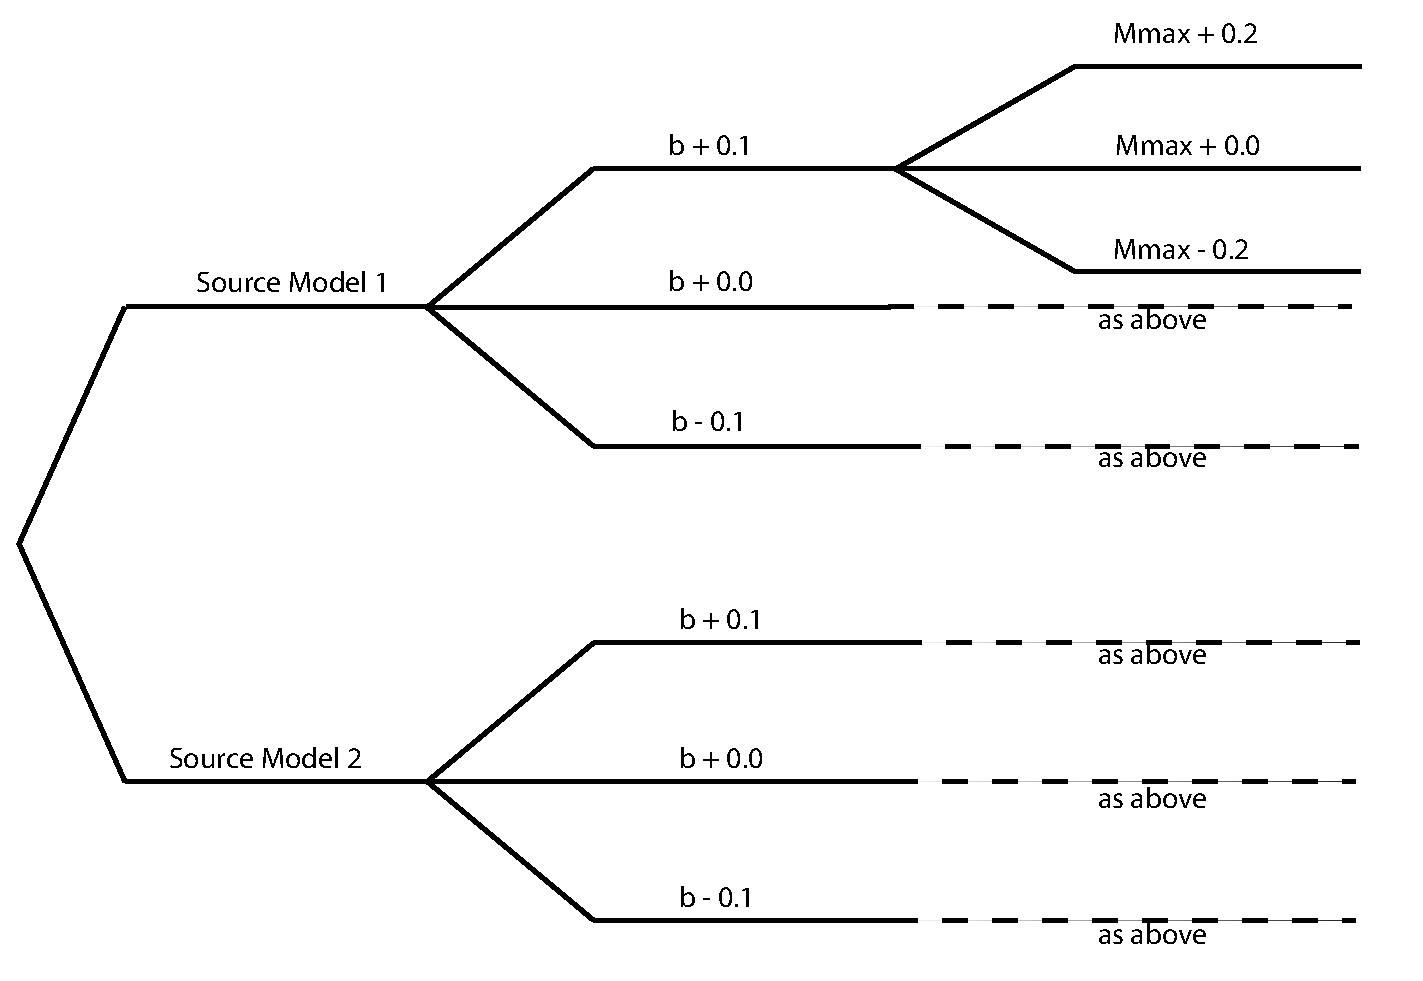
\includegraphics[width=15cm]{./Figures/Part_Hazard/SourceModelLogicTree.eps}
\pstree[treemode=R,levelsep=23ex]{\Tr{}}{
    \pstree{\Tr{\parbox[b]{2.9cm}{Initial seismic sources model 1} }}{
            \pstree{\Tr{  \parbox[b]{1cm}{b-0.1}  }}{
            	\Tr{ \parbox[b]{2cm}{mmax-0.2} }
            	\Tr{ \parbox[b]{2cm}{mmax} }
            	\Tr{ \parbox[b]{2cm}{mmax+0.2} }
    		}
            \pstree{\Tr{ \parbox[b]{1cm}{b} }}{
            	\Tr{ \parbox[b]{2cm}{as above} }
    		}
            \pstree{\Tr{ \parbox[b]{1cm}{b+0.1} }}{
            	\Tr{ \parbox[b]{2cm}{as above} }
    		}
    }
    \pstree{\Tr{\parbox[b]{2.9cm}{Initial seismic sources model 2} }}{
            \pstree{\Tr{ \parbox[b]{1cm}{b-0.1} }}{
            	\Tr{ \parbox[b]{2cm}{as above} }
    		}
            \pstree{\Tr{ \parbox[b]{1cm}{b}}}{
            	\Tr{ \parbox[b]{2cm}{as above} }
    		}
            \pstree{\Tr{ \parbox[b]{1cm}{b+0.1} }}{
            	\Tr{ \parbox[b]{2cm}{as above} }
    		}
    }                 
}
\hfill \\
\caption{Example of Seismic Sources Logic Tree. The first branching level defines
two alternative source models (Source Model 1, Source Model 2). The second 
branching level defines uncertainties in b value (increment of 0.1, 0.0, -0.1).
The third branching level defines uncertainties in maximum magnitude 
(increments of 0.2, 0.0, -0.2).}
\label{fig:SourceModelLogicTree}
\end{figure}
% . . . . . . . . . . . . . . . . . . . . . . . . . . . . . . . . . . . < Figure
% ..............................................................................
%
% . . . . . . . . . . . . . . . . . . . . . . . . . . . . . . . . . . . . . . .
\subsubsection{Supported branch set typologies}
The current version of OpenQuake offers only two built-in typologies of 
branch set. They are only a sample of possible source model epistemic 
uncertainties, and future versions of OpenQuake will provide a broader 
spectrum of built-in epistemic uncertainties. 
%
Currently, rules are applied to all sources. Option to apply rules only 
to specific sources will be also supported in the future.

Figure \ref{fig:SourceModelLogicTree} depicts a source model logic tree that 
can be defined with the options currently present in OpenQuake.
%
\paragraph{Gutenberg-Richter b value uncertainties}
The user can specify a set of increments (positive or negative) that are 
added to Gutenberg-Richter b values. Conservation of total moment rate 
is assumed.
%
\paragraph{Gutenberg-Richter maximum magnitude uncertainties}
The user can specify a set of increments (positive or negative) that are 
added to Gutenberg-Richter maximum magnitude values. 
Conservation of total moment rate is assumed.